\begin{frame}[fragile]\frametitle{Review: Where Matrices Come From}
  \begin{itemize}
    \item System: $2x + 3y = 5$ and $6x + y = 9$
    \item Matrix form: $\begin{pmatrix} 2 & 3 \\ 6 & 1 \end{pmatrix} \begin{pmatrix} x \\ y \end{pmatrix} = \begin{pmatrix} 5 \\ 9 \end{pmatrix}$
    \item Transformation representation
    \item Coefficients organized in rectangular array
    \item Left matrix: transformation
    \item Middle: vector being transformed
    \item Right: result after transformation
  \end{itemize}
\end{frame}

\begin{frame}[fragile]\frametitle{Matrix Notation Basics}
  \begin{itemize}
    \item Order: $m \times n$ (rows $\times$ columns)
    \item Example: $\begin{pmatrix} 2 & 3 \\ 6 & 1 \end{pmatrix}$ is $2 \times 2$
    \item Multiplication rule: columns of first = rows of second
    \item $A_{m \times n} \cdot B_{n \times p} = C_{m \times p}$
    \item Result: first matrix rows, second matrix columns
    \item Order matters: $AB \neq BA$ in general
    \item Non-commutative operation
  \end{itemize}
\end{frame}

\begin{frame}[fragile]\frametitle{Types of Matrices}
  \begin{itemize}
    \item \textbf{Square matrix}: rows = columns ($n \times n$)
    \item Example: $\begin{pmatrix} a & b \\ c & d \end{pmatrix}$ is $2 \times 2$
    \item \textbf{Column matrix}: $\begin{pmatrix} x \\ y \end{pmatrix}$ ($n \times 1$)
    \item \textbf{Row matrix}: $\begin{pmatrix} x & y \end{pmatrix}$ ($1 \times n$)
    \item \textbf{Identity matrix}: special square matrix
    \item Diagonal ones, zeros elsewhere
  \end{itemize}
\end{frame}

\begin{frame}[fragile]\frametitle{Identity Matrix}
  \begin{itemize}
    \item $2 \times 2$ identity: $I_2 = \begin{pmatrix} 1 & 0 \\ 0 & 1 \end{pmatrix}$
    \item $3 \times 3$ identity: $I_3 = \begin{pmatrix} 1 & 0 & 0 \\ 0 & 1 & 0 \\ 0 & 0 & 1 \end{pmatrix}$
    \item Property: $AI = IA = A$ (multiplicative identity)
    \item Like multiplying by 1 in regular numbers
    \item Denoted $I_n$ for $n \times n$ identity
    \item Built from basis vectors
  \end{itemize}
\end{frame}

\begin{frame}[fragile]\frametitle{Basis Vectors}
  \begin{columns}
    \begin{column}[T]{0.6\linewidth}
      \begin{itemize}
        \item 2D basis: $\mathbf{e}_1 = \begin{pmatrix} 1 \\ 0 \end{pmatrix}$, $\mathbf{e}_2 = \begin{pmatrix} 0 \\ 1 \end{pmatrix}$
        \item Same as $\hat{i}$ and $\hat{j}$ unit vectors
        \item Any vector: linear combination of basis
        \item $(2, 3) = 2\begin{pmatrix} 1 \\ 0 \end{pmatrix} + 3\begin{pmatrix} 0 \\ 1 \end{pmatrix}$
        \item Basis vectors span the space
        \item Identity matrix columns are basis vectors
      \end{itemize}
    \end{column}
    \begin{column}[T]{0.4\linewidth}
      \begin{center}
        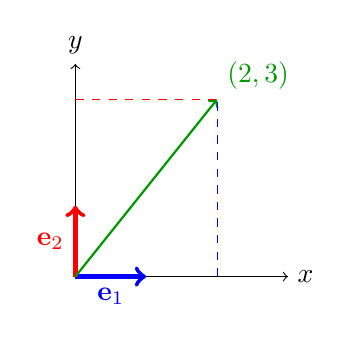
\begin{tikzpicture}[scale=0.9]
          \draw[->] (0,0) -- (3,0) node[right] {$x$};
          \draw[->] (0,0) -- (0,3) node[above] {$y$};
          \draw[->,blue,ultra thick] (0,0) -- (1,0) node[midway,below] {$\mathbf{e}_1$};
          \draw[->,red,ultra thick] (0,0) -- (0,1) node[midway,left] {$\mathbf{e}_2$};
          \draw[->,green!60!black,thick] (0,0) -- (2,2.5) node[above right] {$(2,3)$};
          \draw[dashed,blue] (2,0) -- (2,2.5);
          \draw[dashed,red] (0,2.5) -- (2,2.5);
        \end{tikzpicture}
      \end{center}
    \end{column}
  \end{columns}
\end{frame}

\begin{frame}[fragile]\frametitle{Vector Representation}
  \begin{itemize}
    \item Point $(a, b)$ written as: $\begin{pmatrix} a \\ b \end{pmatrix}$
    \item Equivalently: $a\begin{pmatrix} 1 \\ 0 \end{pmatrix} + b\begin{pmatrix} 0 \\ 1 \end{pmatrix}$
    \item Example: $\begin{pmatrix} -2/3 \\ -5/2 \end{pmatrix} = -\frac{2}{3}\begin{pmatrix} 1 \\ 0 \end{pmatrix} - \frac{5}{2}\begin{pmatrix} 0 \\ 1 \end{pmatrix}$
    \item Same point, different notations
    \item Basis-independent concept
    \item Extension to higher dimensions natural
  \end{itemize}
\end{frame}

\begin{frame}[fragile]\frametitle{Transpose Operation}
  \begin{itemize}
    \item Transpose: rows become columns
    \item Notation: $A^T$ (A transpose)
    \item Example: $\begin{pmatrix} a & b \end{pmatrix}^T = \begin{pmatrix} a \\ b \end{pmatrix}$
    \item $\begin{pmatrix} a & b \\ c & d \end{pmatrix}^T = \begin{pmatrix} a & c \\ b & d \end{pmatrix}$
    \item Order changes: $(m \times n)^T = (n \times m)$
    \item Double transpose returns original: $(A^T)^T = A$
  \end{itemize}
\end{frame}

\begin{frame}[fragile]\frametitle{Symmetric Matrices}
  \begin{itemize}
    \item Definition: $A^T = A$
    \item Transpose equals original
    \item Example: $\begin{pmatrix} 1 & 2 \\ 2 & 1 \end{pmatrix}$
    \item Check: transpose gives same matrix
    \item \textbf{Skew-symmetric}: $A^T = -A$
    \item Example: $\begin{pmatrix} 0 & 2 \\ -2 & 0 \end{pmatrix}$
    \item Important in physics and quantum mechanics
  \end{itemize}
\end{frame}

\begin{frame}[fragile]\frametitle{Complex Numbers: The Argand Plane}
  \begin{columns}
    \begin{column}[T]{0.6\linewidth}
      \begin{itemize}
        \item Real axis (horizontal)
        \item Imaginary axis (vertical)
        \item Point: $z = a + ib$
        \item $a$: real part, $b$: imaginary part
        \item $i = \sqrt{-1}$ (imaginary unit)
        \item Two-dimensional number system
        \item Not the same as 2D space vectors
      \end{itemize}
    \end{column}
    \begin{column}[T]{0.4\linewidth}
      \begin{center}
        \begin{tikzpicture}[scale=0.8]
          \draw[->] (-2,0) -- (3,0) node[right] {Real};
          \draw[->] (0,-2) -- (0,3) node[above] {Imaginary};
          \foreach \x in {-1,1,2}
            \draw (\x,0.1) -- (\x,-0.1) node[below] {\tiny$\x$};
          \foreach \y in {1,2}
            \draw (0.1,\y) -- (-0.1,\y) node[left] {\tiny$\y i$};
          \draw[->,thick,blue] (0,0) -- (2,1.5) node[right] {$2+1.5i$};
          \fill (2,1.5) circle (2pt);
        \end{tikzpicture}
      \end{center}
    \end{column}
  \end{columns}
\end{frame}

\begin{frame}[fragile]\frametitle{Complex Number Operations}
  \begin{itemize}
    \item Addition: $(a+ib) + (c+id) = (a+c) + i(b+d)$
    \item Component-wise addition
    \item Multiplication by real: $k(a+ib) = ka + ikb$
    \item Scaling operation
    \item Multiplication by $-1$: rotate 180°
    \item $(a+ib) \to (-a-ib)$
    \item Multiplication by $i$: rotate 90°
    \item $(a+ib) \cdot i = -b + ia$
  \end{itemize}
\end{frame}

\begin{frame}[fragile]\frametitle{Rotation Interpretation}
  \begin{columns}
    \begin{column}[T]{0.6\linewidth}
      \begin{itemize}
        \item Start at 2 on real axis
        \item Multiply by $-1$: reach $-2$ (180°)
        \item Multiply by $i$: reach $2i$ (90° up)
        \item Multiply by $-i$: reach $-2i$ (90° down)
        \item $i$ represents 90° counterclockwise
        \item $-1$ represents 180° rotation
        \item Foundation for exponential form
      \end{itemize}
    \end{column}
    \begin{column}[T]{0.4\linewidth}
      \begin{center}
        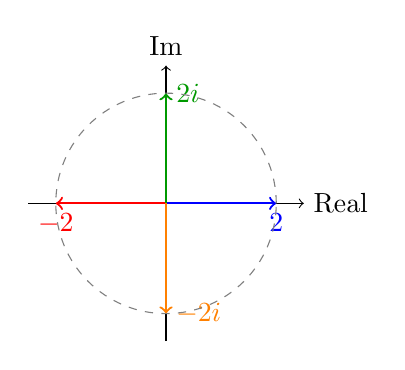
\begin{tikzpicture}[scale=0.7]
          \draw[->] (-2.5,0) -- (2.5,0) node[right] {Real};
          \draw[->] (0,-2.5) -- (0,2.5) node[above] {Im};
          \draw[->,blue,thick] (0,0) -- (2,0) node[below] {$2$};
          \draw[->,red,thick] (0,0) -- (-2,0) node[below] {$-2$};
          \draw[->,green!60!black,thick] (0,0) -- (0,2) node[right] {$2i$};
          \draw[->,orange,thick] (0,0) -- (0,-2) node[right] {$-2i$};
          \draw[gray,dashed] (0,0) circle (2);
        \end{tikzpicture}
      \end{center}
    \end{column}
  \end{columns}
\end{frame}

\begin{frame}[fragile]\frametitle{Euler's Formula}
  \begin{columns}
    \begin{column}[T]{0.6\linewidth}
      \begin{itemize}
        \item \textbf{Euler's formula}: $e^{i\theta} = \cos\theta + i\sin\theta$
        \item Most beautiful equation in mathematics
        \item Connects exponentials, trig, complex numbers
        \item Special case ($\theta = \pi$): $e^{i\pi} = -1$
        \item Euler's identity: $e^{i\pi} + 1 = 0$
        \item Contains $e, i, \pi, 1, 0$ — fundamental constants
      \end{itemize}
    \end{column}
    \begin{column}[T]{0.4\linewidth}
      \begin{center}
        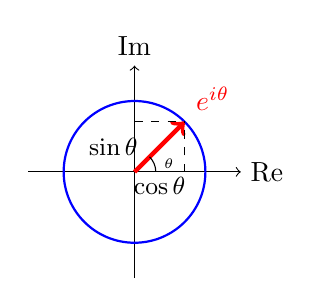
\begin{tikzpicture}[scale=0.9]
          \draw[->] (-1.5,0) -- (1.5,0) node[right] {Re};
          \draw[->] (0,-1.5) -- (0,1.5) node[above] {Im};
          \draw[blue,thick] (0,0) circle (1);
          \draw[->,red,ultra thick] (0,0) -- ({cos(45)},{sin(45)}) node[above right] {$e^{i\theta}$};
          \draw[dashed] ({cos(45)},0) -- ({cos(45)},{sin(45)});
          \draw[dashed] (0,{sin(45)}) -- ({cos(45)},{sin(45)});
          \node at ({cos(45)/2},-0.2) {\small $\cos\theta$};
          \node at (-0.3,{sin(45)/2}) {\small $\sin\theta$};
          \draw (0.3,0) arc (0:45:0.3) node[midway,right] {\tiny $\theta$};
        \end{tikzpicture}
      \end{center}
    \end{column}
  \end{columns}
\end{frame}

\begin{frame}[fragile]\frametitle{Euler's Identity Derivation}
  \begin{itemize}
    \item Taylor series: $e^x = 1 + x + \frac{x^2}{2!} + \frac{x^3}{3!} + \cdots$
    \item Substitute $x = i\theta$: $e^{i\theta} = 1 + i\theta + \frac{(i\theta)^2}{2!} + \frac{(i\theta)^3}{3!} + \cdots$
    \item Note: $i^2 = -1$, $i^3 = -i$, $i^4 = 1$
    \item Separate real and imaginary: $e^{i\theta} = \left(1 - \frac{\theta^2}{2!} + \frac{\theta^4}{4!} - \cdots\right) + i\left(\theta - \frac{\theta^3}{3!} + \frac{\theta^5}{5!} - \cdots\right)$
    \item Recognize: $\cos\theta = 1 - \frac{\theta^2}{2!} + \frac{\theta^4}{4!} - \cdots$
    \item And: $\sin\theta = \theta - \frac{\theta^3}{3!} + \frac{\theta^5}{5!} - \cdots$
    \item Therefore: $e^{i\theta} = \cos\theta + i\sin\theta$
  \end{itemize}
\end{frame}

\begin{frame}[fragile]\frametitle{Three Forms of Complex Numbers}
  \begin{itemize}
    \item \textbf{Cartesian (algebraic)}: $z = a + ib$
    \item Gives real and imaginary parts directly
    \item \textbf{Polar}: $z = r(\cos\theta + i\sin\theta)$
    \item $r$: magnitude (distance from origin)
    \item $\theta$: argument (angle from positive real axis)
    \item \textbf{Exponential}: $z = re^{i\theta}$
    \item Most compact and powerful form
    \item All three represent the same number
  \end{itemize}
\end{frame}

\begin{frame}[fragile]\frametitle{Converting Between Forms}
  \begin{itemize}
    \item Example: Convert $1 + i$ to other forms
    \item Magnitude: $r = \sqrt{1^2 + 1^2} = \sqrt{2}$
    \item Angle: $\tan\theta = \frac{1}{1} = 1 \Rightarrow \theta = \frac{\pi}{4}$
    \item Polar: $\sqrt{2}\left(\cos\frac{\pi}{4} + i\sin\frac{\pi}{4}\right)$
    \item Exponential: $\sqrt{2}e^{i\pi/4}$
    \item Formula: $a + ib \to re^{i\theta}$ where $r = \sqrt{a^2+b^2}$, $\theta = \arctan(b/a)$
  \end{itemize}
\end{frame}

\begin{frame}[fragile]\frametitle{Complex Conjugate}
  \begin{itemize}
    \item Definition: conjugate of $a + ib$ is $a - ib$
    \item Notation: $\overline{z}$ or $z^*$
    \item Geometric: reflection across real axis
    \item Example: $\overline{2 + 3i} = 2 - 3i$
    \item Property: $z \cdot \overline{z} = a^2 + b^2 = |z|^2$
    \item Gives magnitude squared
    \item Modulus: $|a + ib| = \sqrt{a^2 + b^2}$
  \end{itemize}
\end{frame}

\begin{frame}[fragile]\frametitle{Hermitian Conjugate}
  \begin{itemize}
    \item For matrices with complex entries
    \item Hermitian conjugate: transpose + conjugate
    \item Notation: $A^\dagger$ (A dagger)
    \item Operation: $(A^\dagger)_{ij} = \overline{A_{ji}}$
    \item Example: $\begin{pmatrix} 2 & 1+i \\ 3i & 1 \end{pmatrix}^\dagger = \begin{pmatrix} 2 & -3i \\ 1-i & 1 \end{pmatrix}$
    \item Order: transpose then conjugate (or vice versa)
    \item Essential for quantum mechanics
  \end{itemize}
\end{frame}

\begin{frame}[fragile]\frametitle{Hermitian Matrices}
  \begin{itemize}
    \item Definition: $A^\dagger = A$
    \item Hermitian conjugate equals original
    \item Example: $\begin{pmatrix} 0 & i \\ -i & 0 \end{pmatrix}$
    \item Check: transpose gives $\begin{pmatrix} 0 & -i \\ i & 0 \end{pmatrix}$
    \item Conjugate: $\begin{pmatrix} 0 & i \\ -i & 0 \end{pmatrix}$ (original)
    \item \textbf{Skew-Hermitian}: $A^\dagger = -A$
    \item Hermitian matrices: observables in QM
    \item Real eigenvalues guaranteed
  \end{itemize}
\end{frame}

\begin{frame}[fragile]\frametitle{Unitary Matrices}
  \begin{itemize}
    \item Definition: $A^\dagger A = I$
    \item Hermitian conjugate times matrix = identity
    \item Complex analog of orthogonal matrices
    \item Example: identity matrix $I = \begin{pmatrix} 1 & 0 \\ 0 & 1 \end{pmatrix}$
    \item Check: $I^\dagger I = I \cdot I = I$
    \item Unitary transformations preserve inner products
    \item Quantum mechanics: all evolution is unitary
    \item Half of quantum computing based on this
  \end{itemize}
\end{frame}

\begin{frame}[fragile]\frametitle{Eigenvalues and Eigenvectors}
  \begin{itemize}
    \item Eigenvalue equation: $M\mathbf{v} = \lambda\mathbf{v}$
    \item $M$: operator/transformation matrix
    \item $\mathbf{v}$: eigenvector (special vector)
    \item $\lambda$: eigenvalue (scaling factor)
    \item Meaning: transformation only scales, doesn't rotate
    \item Example: stretch by factor $\lambda$ in direction $\mathbf{v}$
    \item $\lambda$ can be real, complex, even imaginary
    \item Fancy German terminology: eigen = "own" or "characteristic"
  \end{itemize}
\end{frame}

\begin{frame}[fragile]\frametitle{Schrödinger Equation}
  \begin{itemize}
    \item Time-dependent: $i\hbar\frac{\partial}{\partial t}|\psi\rangle = \hat{H}|\psi\rangle$
    \item Time-independent: $\hat{H}|\psi\rangle = E|\psi\rangle$
    \item This IS an eigenvalue equation
    \item $\hat{H}$: Hamiltonian operator (energy operator)
    \item $|\psi\rangle$: wave function (eigenvector)
    \item $E$: energy (eigenvalue)
    \item Solves for allowed energies and states
    \item Foundation of quantum mechanics
  \end{itemize}
\end{frame>

\begin{frame}[fragile]\frametitle{Summary}
  \begin{itemize}
    \item Matrices: organized arrays of numbers
    \item Basis vectors: building blocks of space
    \item Complex numbers: $a + ib$, three forms
    \item Euler's formula: $e^{i\theta} = \cos\theta + i\sin\theta$
    \item Conjugate: flip imaginary sign
    \item Hermitian: $A^\dagger = A$ (observables)
    \item Unitary: $A^\dagger A = I$ (evolution)
    \item Eigenvalues: measurement outcomes
    \item All pieces ready for quantum mechanics
  \end{itemize}
\end{frame}
